\documentclass{standalone}
\usepackage{tikz}

\begin{document}
\begin{minipage}{0.75\textwidth}
	\centering
	\scalebox{0.7}{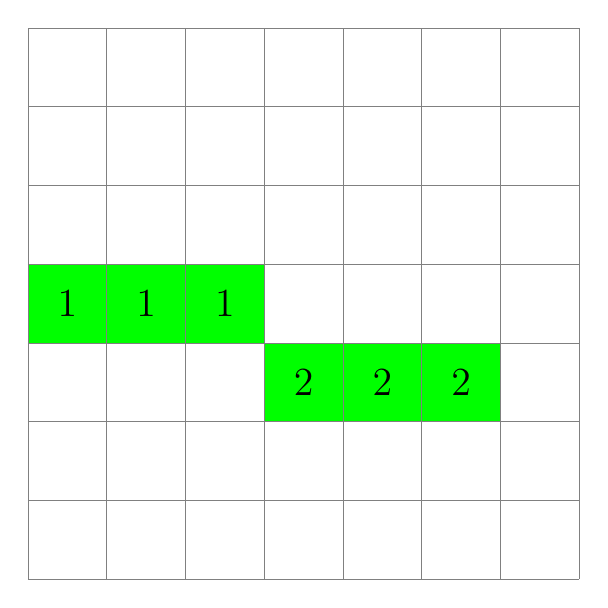
\begin{tikzpicture}

	\foreach \x in {0,1,2}
	\fill[green] (-1+\x,3) rectangle (0+\x,4);  
	\foreach \x in {0,1,2}
	\fill[green] (2+\x,2) rectangle (3+\x,3);   
	\draw[step=1cm,gray,very thin] (-1,-0) grid (6,7);

	\node at (-0.5,3.5) {\Large{1}}; 
	\node at (0.5,3.5) {\Large{1}}; 
	\node at (1.5,3.5) {\Large{1}}; 
	\node at (2.5,2.5) {\Large{2}}; 
	\node at (3.5,2.5) {\Large{2}}; 
	\node at (4.5,2.5) {\Large{2}}; 
	\end{tikzpicture}}
	\hspace{1cm}
	\scalebox{0.7}{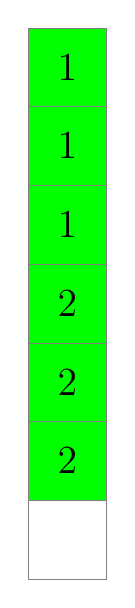
\begin{tikzpicture}
		\foreach \x in {1,2,3,4,5,6}
		\fill[green] (8,\x) rectangle (9,\x+1);  
		\draw[step=1cm,gray,very thin] (8,-0) grid (9,7);
		\node at (8.5,6.5) {\Large{1}}; 
		\node at (8.5,5.5) {\Large{1}}; 
		\node at (8.5,4.5) {\Large{1}}; 
		\node at (8.5,3.5) {\Large{2}}; 
		\node at (8.5,2.5) {\Large{2}}; 
		\node at (8.5,1.5) {\Large{2}}; 
		\end{tikzpicture}}
\end{minipage}
\end{document}
